\documentclass[a4paper]{article}
\usepackage{graphicx}
\title{Tutorial Composition and Idioms}
\author{Francis Bond \url{<bond@ieee.org>}}
\date{}%2011-08-15}
\usepackage{fontenc}
\usepackage{polyglossia}
\setmainlanguage{english}
\setmainfont{TeX Gyre Pagella}
\setsansfont[Ligatures=TeX]{TeX Gyre Heros}
\usepackage{xeCJK}
\setCJKmainfont{Noto Sans CJK JP}
\setCJKsansfont{Noto Sans CJK JP}
\setCJKmonofont{Noto Sans CJK JP}
%\newcommand{\ans}[1]{\hfill{#1}}
%\newcommand{\ans}[1]{}
%%% dynamically add answers
\input{answers}

\usepackage{xspace}
\newcommand{\ent}{\ensuremath{\Rightarrow}\xspace}
\newcommand{\nent}{\ensuremath{\not\Rightarrow}\xspace}
\newcommand{\Y}[1]{\textbf{#1}}

\usepackage{multicol}
%\Restriction{}
%\rightfooter{}
%\leftheader{}
%\rightheader{}
\usepackage{mygb4e}
\usepackage[e,j]{mtg2e}
\newcommand{\lex}[1]{\textbf{\textit{#1}}}
\newcommand{\lx}[1]{\textbf{\textit{#1}}}
\newcommand{\ix}{\ex\it}
%\newcommand{\eng}{\textit}
\newcommand{\con}[1]{\textsc{#1}}
\usepackage{url}
\usepackage[normalem]{ulem}
\newcommand{\ul}[1]{\uline{#1}}
\newcommand{\txx}[1]{\textbf{#1}}

\begin{document}
\maketitle
\begin{enumerate}
  \item Consider the following English phrases:
    \begin{enumerate}
    \item walk quickly
      \abox{compositional}
    \item spill the tea
      \abox{non-compositional:  ``reveal gossip or secrets''}
    \item green thumb
      \abox{non-compositional: ``talent for gardening''}
    \item write an email
      \abox{compositional}
    \item night sky
      \abox{compositional}
    \item break the ice
      \abox{non-compositional: ``to initiate social interaction, reduce tension''}
    \end{enumerate}
    Which ones have a non-compositional reading, and what is it?
    \\  e.g. \textit{hit the sack} --- non-compositional: ``go to bed'';\\
    \textit{hit the nail} --- compositional
    
\item Give an example of a multiword expression meaning the following in a language you speak.
  \begin{exe}
    \ex become angry
    \abox{\jpn{hara ga tatsu} (腹が立つ) ``my stomach rises''}
    \ex die
    \abox{\eng{pass away}}
    \ex get up early
    \abox{rise with the lark
    \\ \eng{Vstávat se slepicemi} ``get up with the chickens''}
  \ex do two things at once
  \abox{ \eng{Zabít dvě mouchy jednou ranou} ``kill two flies with one hit''
\\ kill two birds with one stone.}
\ex rain heavily
\abox{\jpn{doshaburi} 土砂降り ``rain eath and sand''
  \\ \eng{rain cats and dogs}
  \\ \eng{Lije jako z konve}  ``raining as if from a watering can''}
  \end{exe}

  \newpage

\item Classify following Czech idioms as
  \begin{enumerate}
  \item Fixed Expression
  \item Semi-Fixed Expression
  \item Decomposable Expression
  \item Non-decomposable Expression
  \item Institutionalized Phrases
  \end{enumerate}
  \begin{exe}
    \ex \eng{házet klacky pod nohy} ``throw sticks under feet'
    \ex \eng{mít máslo na hlavě} ``have butter on head''
    \ex \eng{vzít roha} ``run away''
    \ex \eng{tak říkajíc} ``so to speak''
    \ex \eng{sůl a pepř} ``salt and pepper''
    \ex \eng{zuby nehty} ``tooth and nail''
    \ex \eng{ztratit hlavu} ``lose head''
    \ex \eng{otevřít někomu oči} ``open someone's eyes''
    \ex \eng{v průběhu} ``in progress'' (during)
    \ex \eng{na koleně} ``on knee'' (improvised)
  \end{exe}
  \newpage
\item Enjoy the following example: (thanks to Jindra Rehak)
  
  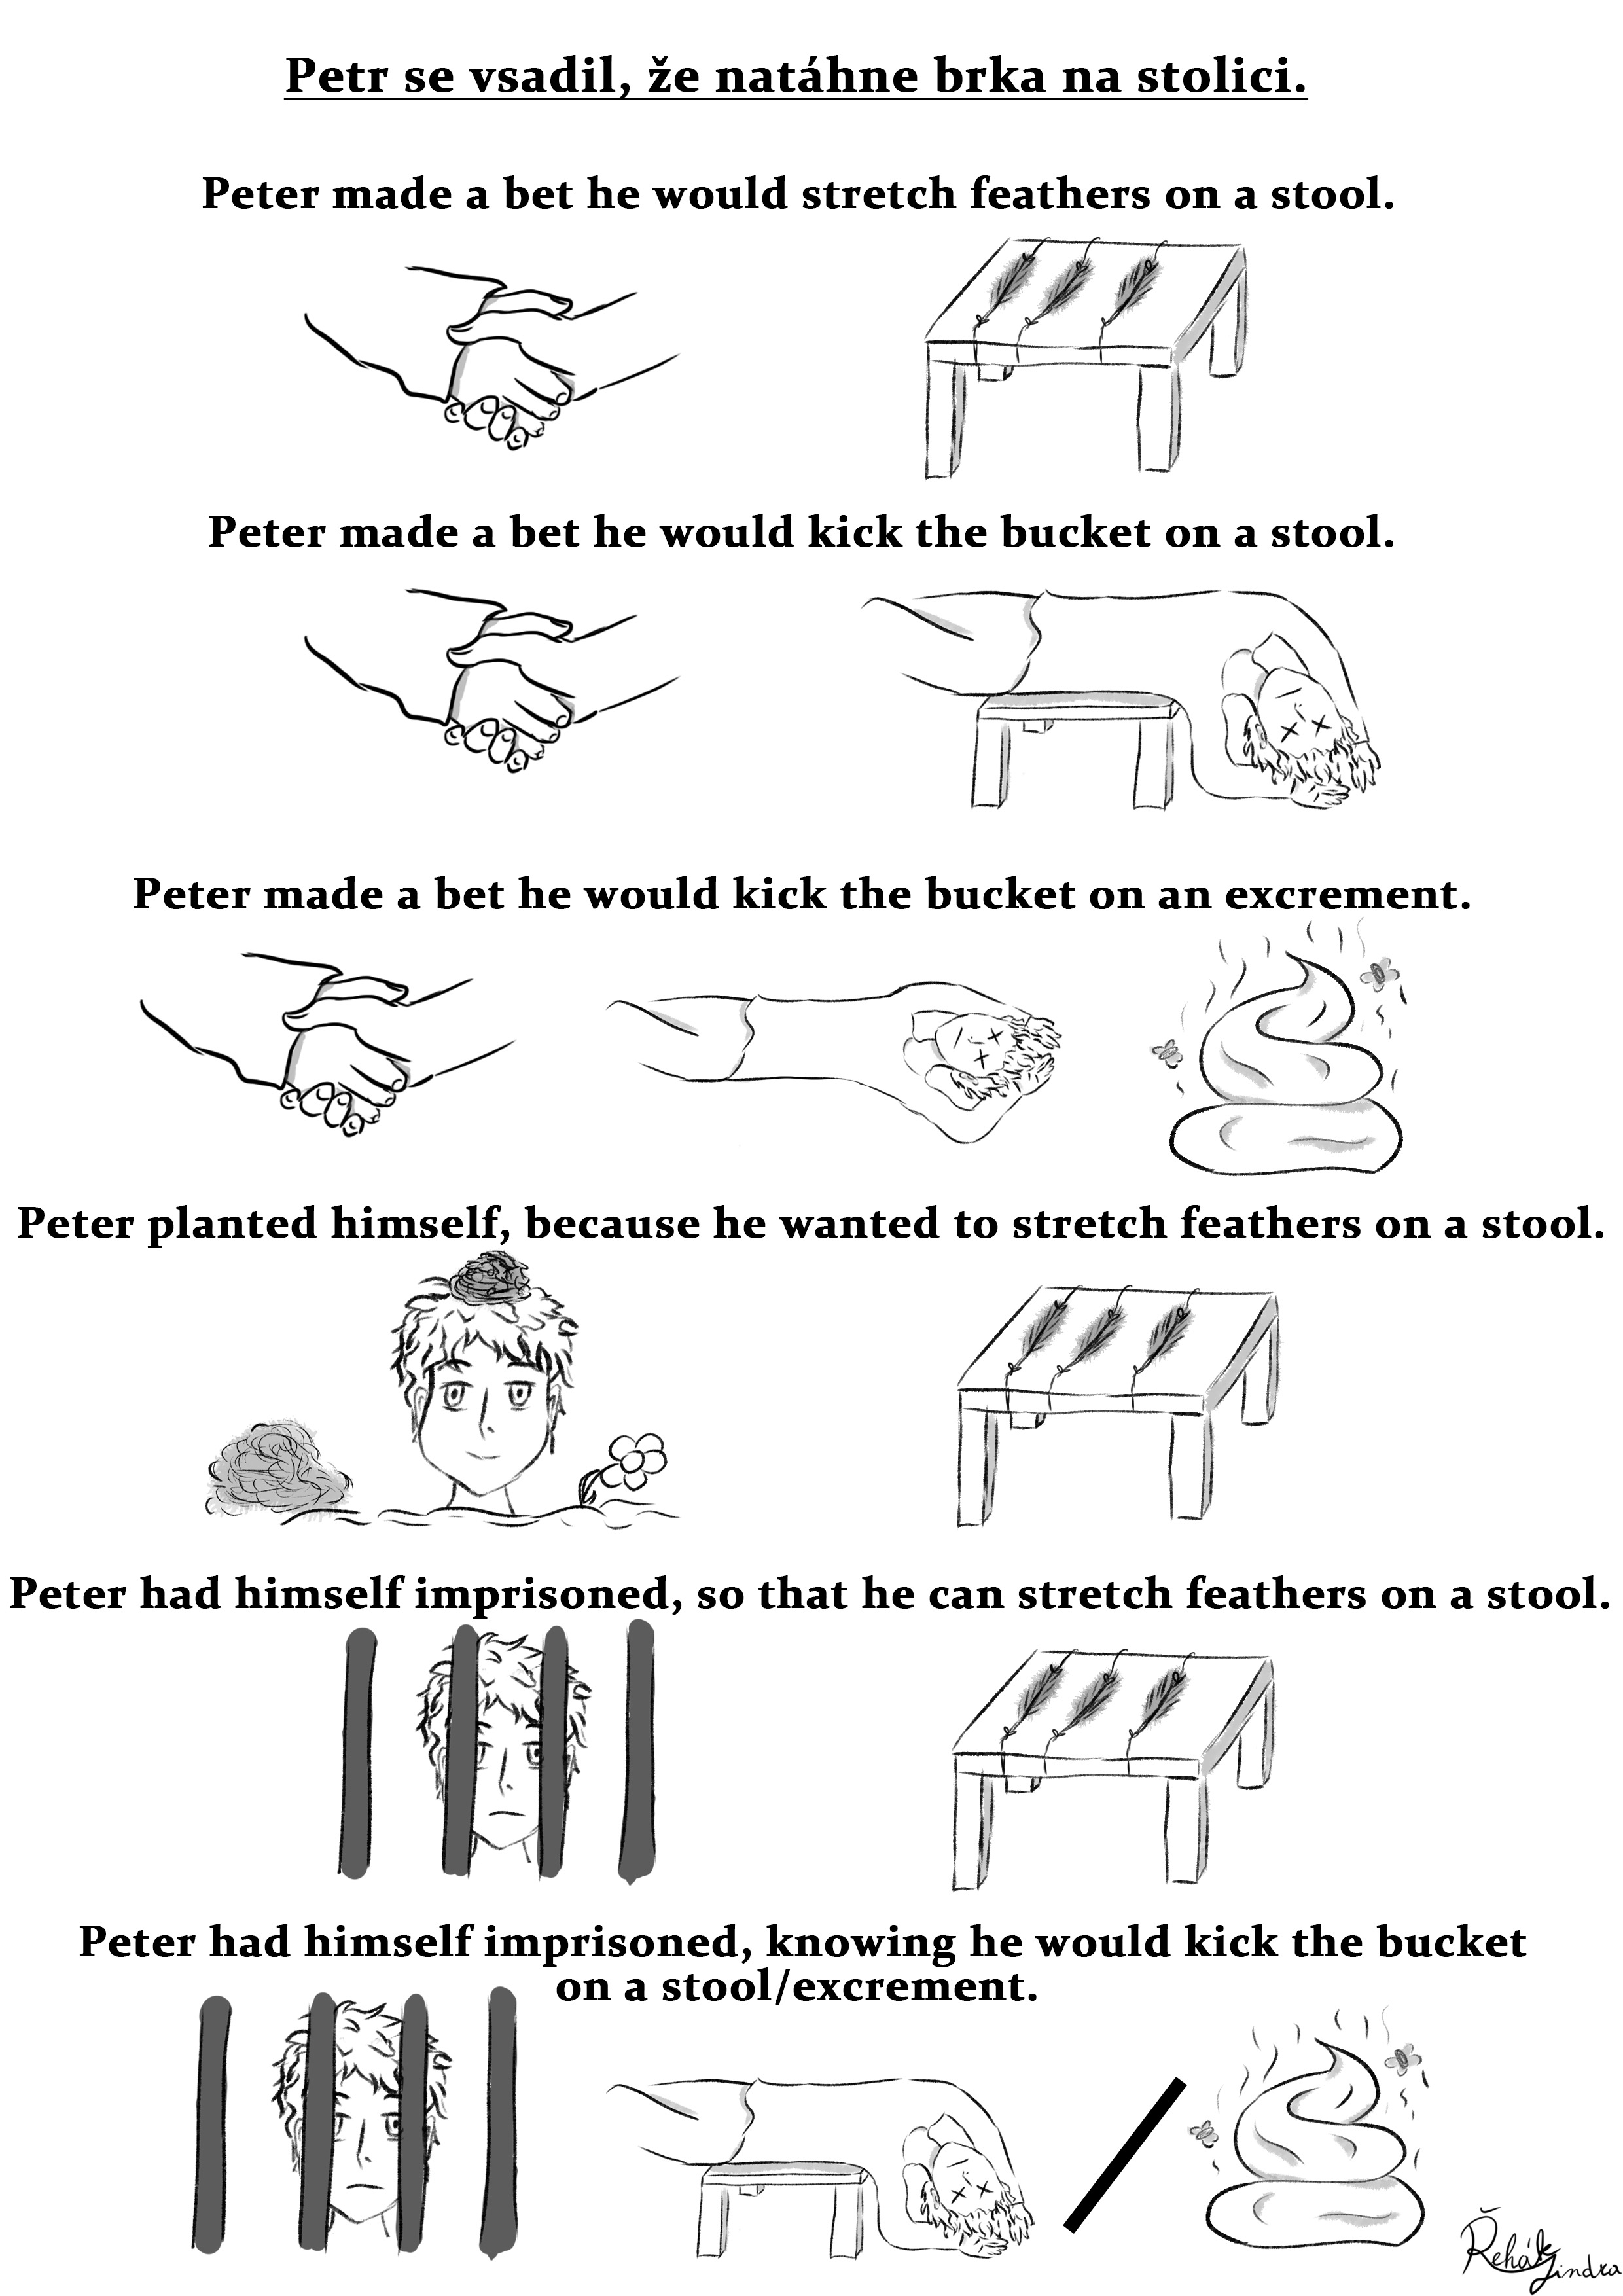
\includegraphics[width=\textwidth]{img/Linguistic Ambiguity in a Czech Sentence - Jindra Rehak.jpg}
\end{enumerate}

\end{document}

%%% Local Variables: 
%%% coding: utf-8
%%% mode: latex
%%% TeX-PDF-mode: t
%%% TeX-engine: xetex
%%% End: 
